\documentclass[a5paper, 12pt, twoside]{scrartcl}

\usepackage[europeanresistors]{circuitikz}
\usepackage{siunitx}
\usepackage{lipsum, mystyle}

\usepackage{scrlayer-scrpage}

\clearpairofpagestyles{}

\setkomafont{pageheadfoot}{\sffamily\footnotesize}
\setkomafont{pagination}{}

\ohead{Seite~\pagemark}
\ihead{Emil Slomka, Tim Hilt}

\KOMAoptions{
  headsepline=true,
}

\begin{document}

\newgeometry{left=1cm, right=1cm, top=2cm, bottom=1cm}
\begin{center}
  \usekomafont{disposition}\huge Elektronik Formelsammlung
\end{center}

{\usekomafont{disposition}\Large 1 Grundlagen und Wiederholung}

\vspace{.5cm}

\begin{minipage}{.48\textwidth}
  \(R_1 || R_2 = \frac{R_1 \cdot R_2}{R_1 + R_2}\)
\end{minipage}\hfill\vline\hfill%
\begin{minipage}{.48\textwidth}
  \textbf{Spannungsquelle in Stromquelle}

  \begin{circuitikz}
    \draw (0,0) -- (3,0) to [R, l=\(R_a\)] (6,0) to [open, o-o] (6,-2.5) -- (0,-2.5) to [european current source, l=\(I_e\)] (0,0);
    \draw (3,0) to [R, l=\(R_i\), *-*] (3,-2.5);
  \end{circuitikz}
  \begin{circuitikz}
    \draw (0,0) to [R, l=\(R_i\)] (3,0) to [R, l=\(R_a\)] (6,0) to [open, o-o] (6,-2.5) -- (0,-2.5) to [european voltage source, l=\(U_e\)] (0,0);
  \end{circuitikz}

  mit
  \[U_e = I_e \cdot R_i\]
  \end{minipage}

\vspace{.5cm}
{\usekomafont{disposition}\Large 2 Kondensator und Zeitkonstanten}
\vspace{.5cm}

Zeitkonstante \(\tau\) beim \mybfcol{Kondensator}: \dotfill \(\tau = R \cdot C\)\\
Zeitkonstante \(\tau\) bei der \mybfcol{Spule}: \dotfill \(\tau = \frac{L}{R}\)\\

\begin{figure}[H]
  \centering
  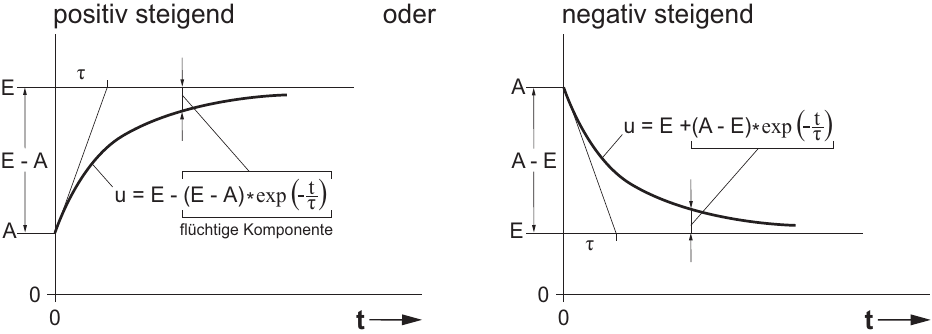
\includegraphics[width=.7\textwidth]{LadekurveKondensator}
  \caption{Ladekurven Kondensator \mybfcol{Achtung: \(t = \Delta t = t_1 - t_0\)}}
\end{figure}

\begin{center}
  \begin{tabular}{ll}
    \toprule
    Wenn Ladung von \SI{0}{\volt} nach \(U_e\): & \(U_a = U_e \cdot (1 - e^{-\frac{t}{\tau}})\)\\
    Wenn Entladung von \(A\) nach \SI{0}{\volt} & \(U_a = U_e \cdot e^{-\frac{t}{\tau}}\)\\
    \bottomrule
  \end{tabular}
\end{center}

\textbf{Zum Zeichnen im Zeitbereich:} Arbeitsgerade von Anfangsspannung zur Endspannung zeichnen, mit \(t = \tau\)

\mybfcol{Achtung: Immer alle Widerstände parallel und in Reihe zum Kondensator berücksichtigen und Übertragungsfunktion für Ladeziel verwenden!}


\begin{table}[H]
  \centering
  \begin{tabular}{cc}
    \toprule
    \(t=\tau\) & \(\approx 63\%\) von\ \(|A-E|\)\\
    \(t=2\tau\) & \(\approx 86\%\) von\ \(|A-E|\)\\
    \(t=5\tau\) & \(\approx 99\%\) von\ \(|A-E|\)\\
    \bottomrule
  \end{tabular}
\end{table}
 
{\usekomafont{disposition}\Large 3 Filter}\\[1em]
Im Fourierbereich: \(\omega = 2 \pi f\), im Laplacebereich: \(j\omega = p\)
\begin{center}
  \begin{tabular}{cllll}
    \toprule
    & \textbf{RC-Tiefpass} & \textbf{RC-Hochpass} & \textbf{RL-Tiefpass} & \textbf{RL-Hochpass}\\
    \midrule
    \textbf{Übertragungsfunktion \(\frac{U_a}{U_e} = H(j\omega)\)} & \(\frac{1}{1 + j\omega R C}\) & \(\frac{j\omega RC}{1 + j\omega RC}\) & \(\frac{R}{R + j \omega L}\)& \(\frac{j\omega L}{R + j \omega L}\) \\[1em]
    \textbf{Grenzfrequenz \(f_G / \omega_G\)} & \(\frac{1}{2 \pi R C}; \frac{1}{RC}\) & \(\frac{1}{2 \pi R C}; \frac{1}{RC}\) & \(\frac{R}{2 \pi L}; \frac{R}{L}\) & \(\frac{R}{2 \pi L}; \frac{R}{L}\)\\
    \bottomrule
  \end{tabular}
\end{center}
\begin{minipage}{.48\linewidth}
  \begin{figure}[H]
    \centering
    \begin{circuitikz}
      \draw (0,0) to [R, l=\(R\)] (4,0) to [C, l_=\(C\)] (4,-2) node[rground]{};
      \draw (0,0) to [european voltage source] (0,-2) node[rground]{};
      \draw (-.5,0) to [open, v=\(U_e\)] (-.5,-2);
      \draw (4.5,0) to [open, v^=\(U_a\)] (4.5,-2);
    \end{circuitikz}
    \caption{RC-Tiefpass}
  \end{figure}
  \begin{figure}[H]
    \centering
    \begin{circuitikz}
      \draw (0,0) to [L, l=\(L\)] (4,0) to [R, l_=\(R\)] (4,-2) node[rground]{};
      \draw (0,0) to [european voltage source] (0,-2) node[rground]{};
      \draw (-.5,0) to [open, v=\(U_e\)] (-.5,-2);
      \draw (4.5,0) to [open, v^=\(U_a\)] (4.5,-2);
    \end{circuitikz}
    \caption{RL-Tiefpass}
  \end{figure}
\end{minipage}\hfill%
\begin{minipage}{.48\linewidth}
  \begin{figure}[H]
    \centering
    \begin{circuitikz}
      \draw (0,0) to [C, l=\(C\)] (4,0) to [R, l_=\(R\)] (4,-2) node[rground]{};
      \draw (0,0) to [european voltage source] (0,-2) node[rground]{};
      \draw (-.5,0) to [open, v=\(U_e\)] (-.5,-2);
      \draw (4.5,0) to [open, v^=\(U_a\)] (4.5,-2);
    \end{circuitikz}
    \caption{RC-Hochpass}
  \end{figure}
  \begin{figure}[H]
    \centering
    \begin{circuitikz}
      \draw (0,0) to [R, l=\(R\)] (4,0) to [L, l_=\(L\)] (4,-2) node[rground]{};
      \draw (0,0) to [european voltage source] (0,-2) node[rground]{};
      \draw (-.5,0) to [open, v=\(U_e\)] (-.5,-2);
      \draw (4.5,0) to [open, v^=\(U_a\)] (4.5,-2);
    \end{circuitikz}
    \caption{RL-Hochpass}
  \end{figure}
\end{minipage}

\textbf{Dämpfung bei passiven Filtern erster Ordnung:}

\begin{itemize}
\item Dämpfung um einen Anfangswert im Durchlassbereich (Muss berechnet werden, indem\\ \(20 \cdot \log(|H(0)|)\) berechnet wird)
\item Anfangswert \(- \SI{3}{\decibel}\) an der Grenzfrequenz \(f_G\)
\item \SI{6}{\decibel} pro Oktave (doppelte Frequenz) im Sperrbereich
\item \SI{20}{\decibel} pro Dekade (zehnfache Frequenz) im Sperrbereich
\end{itemize}

\textbf{Konstruktion von Bode-Diagrammen}

\begin{enumerate}
\item \(|H(f)|\) bestimmen
\item \(f_G\) berechnen
\item Werte für \(f\) in \(|H(f)|\) einsetzen (für \(f=0\) und zwei Werte im Sperrbereich) und \(20\cdot\log(|H(f)|)\) berechnen
\item Asymptoten zeichnen
\item Bode Diagramm zeichnen, \(f_G\) befindet sich am Schnittpunkt beider Asymptoten
\end{enumerate}
\newpage

% --------------------- OPV ---------------------
\begin{figure}[H]
  \centering
  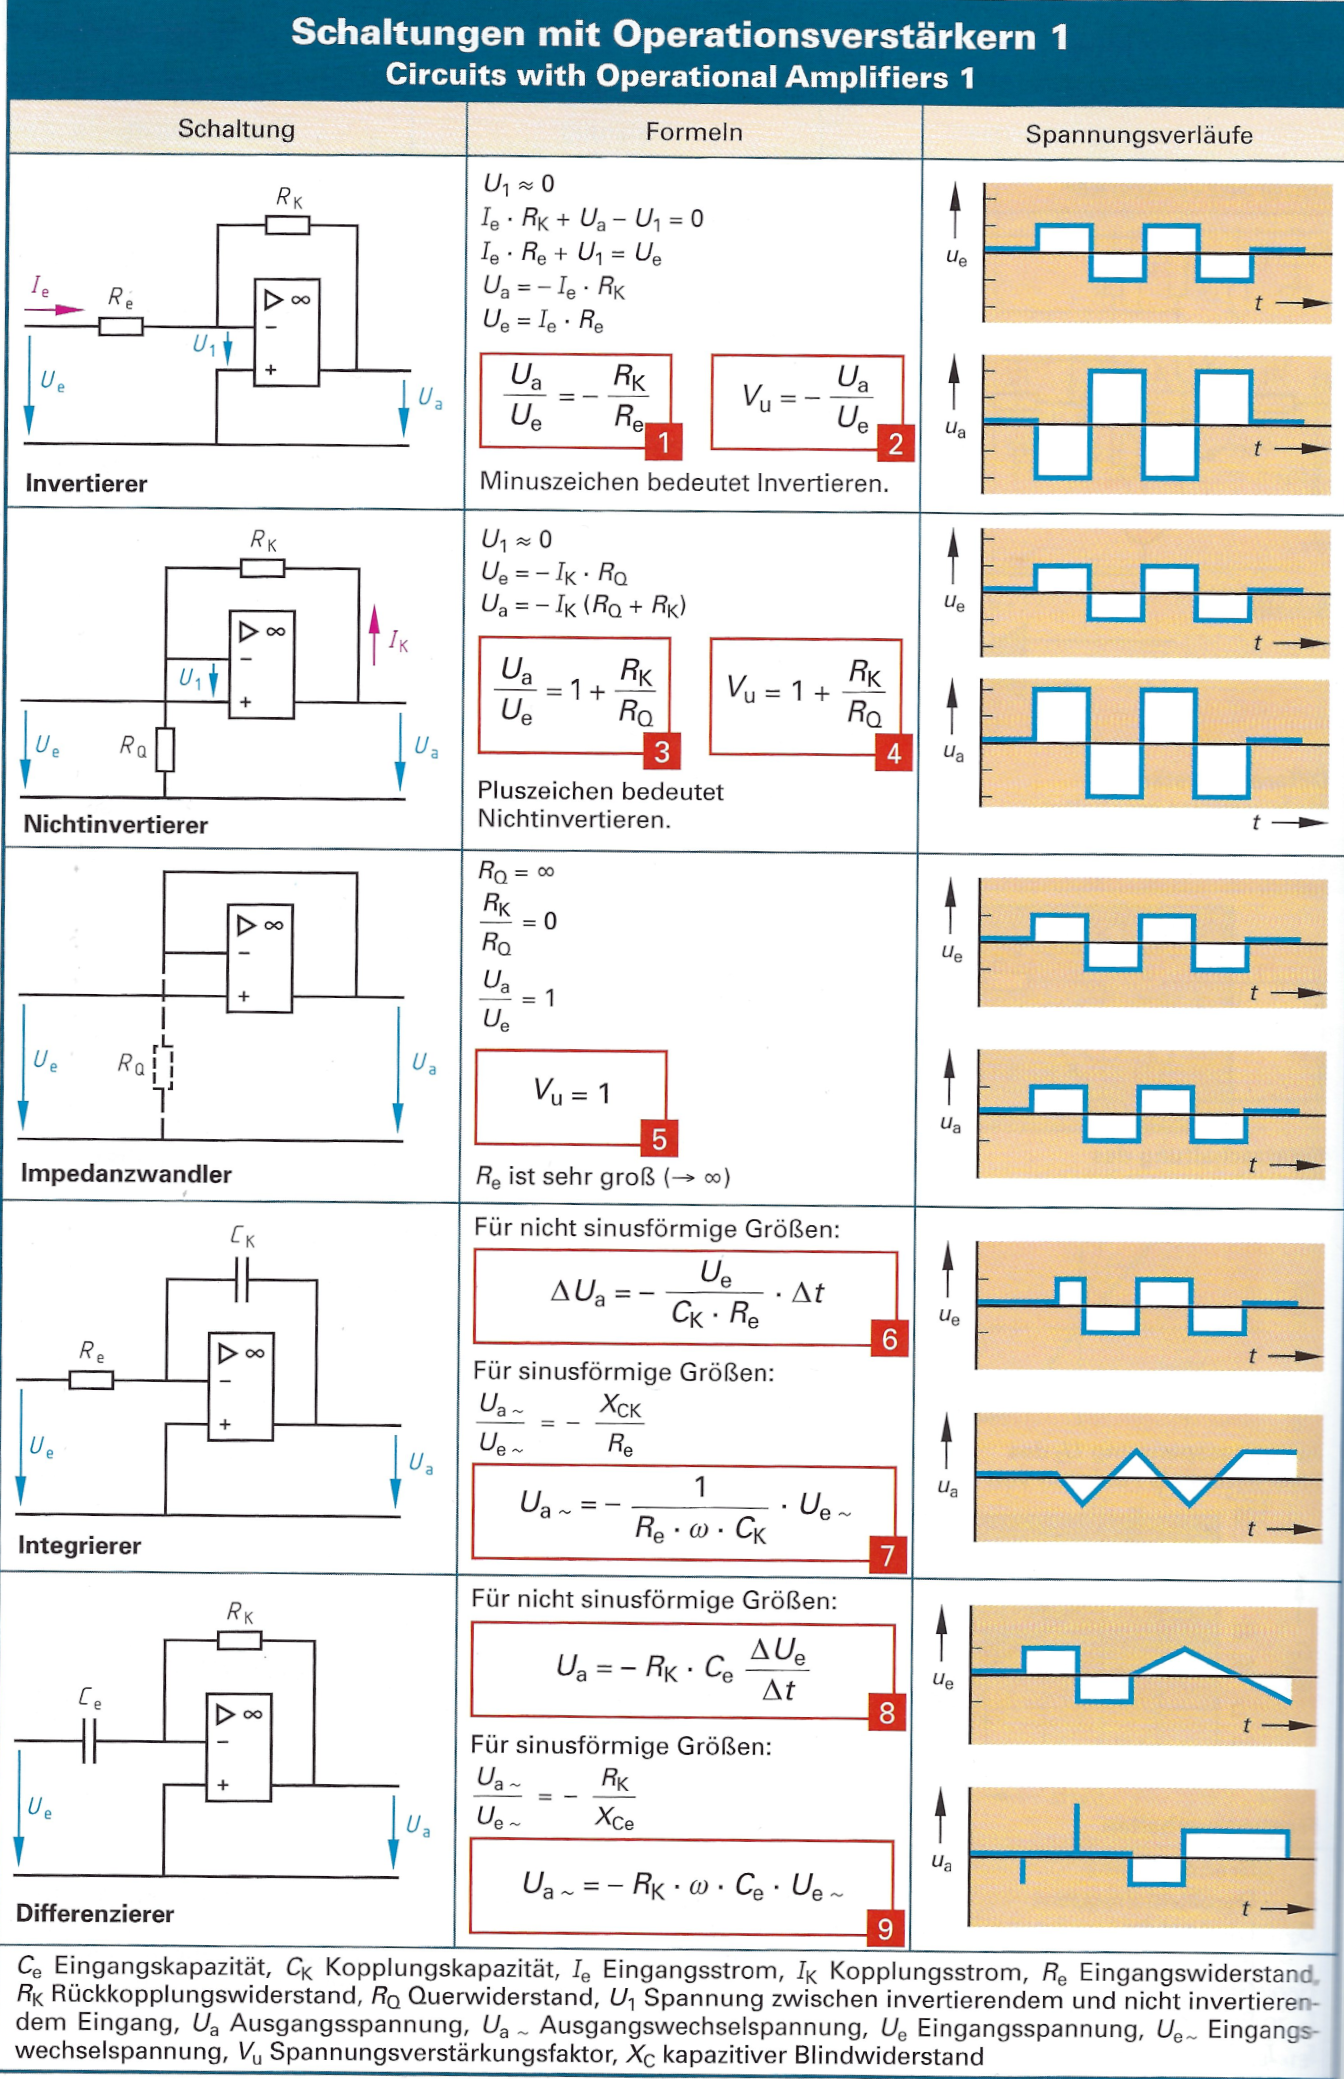
\includegraphics[width=.93\textwidth]{OPV1}
\end{figure}
\begin{figure}[H]
  \centering
  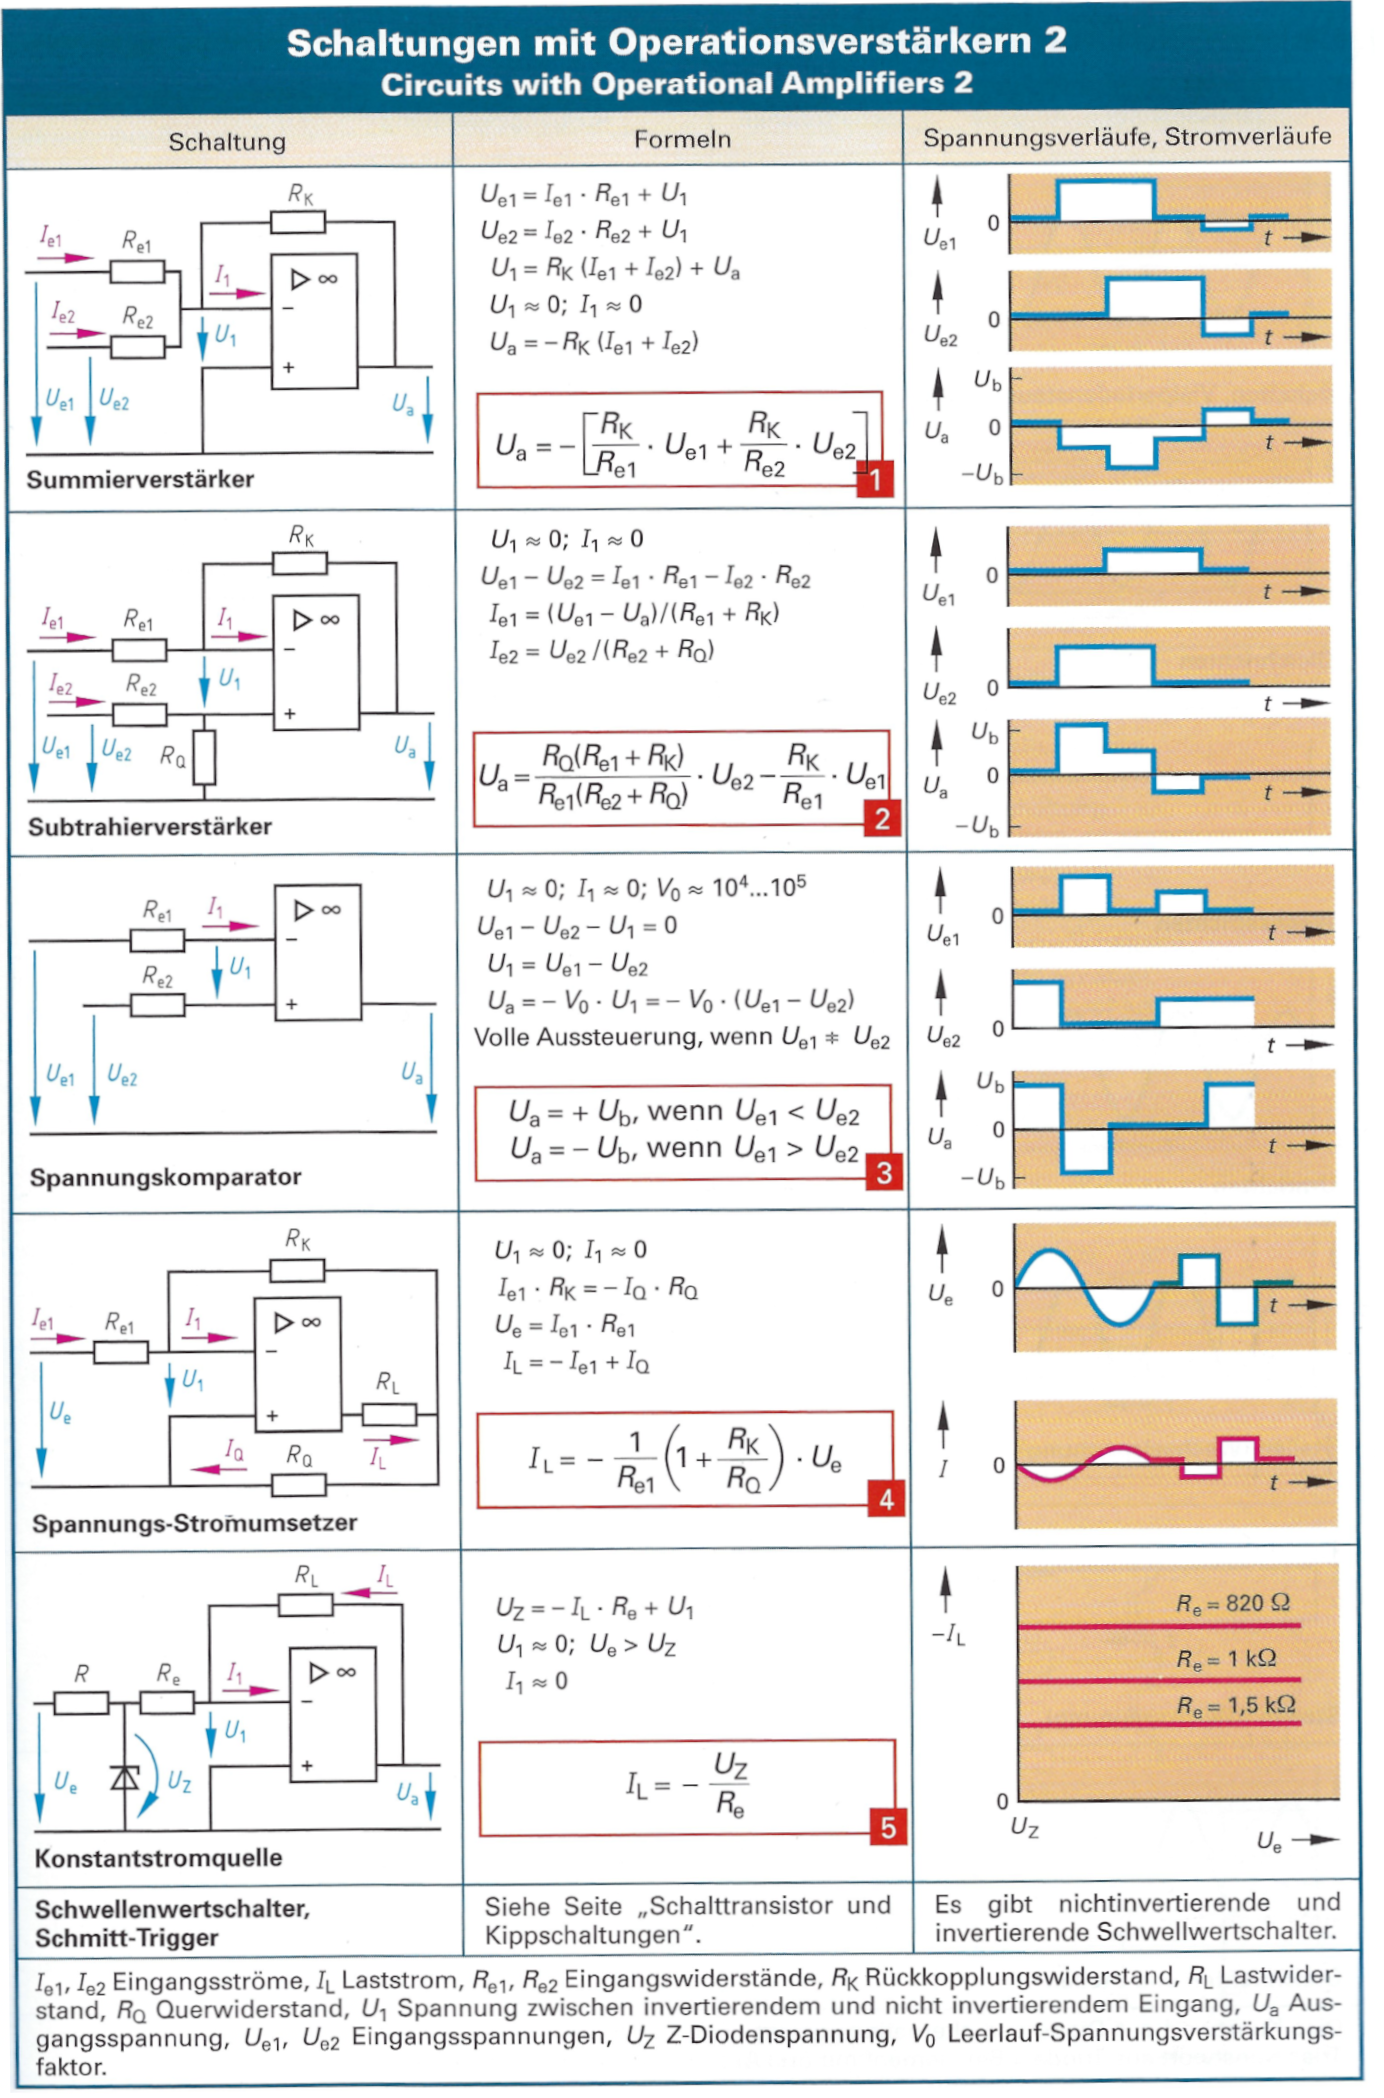
\includegraphics[width=.95\textwidth]{OPV2}
\end{figure}
% -----------------------------------------------

{\usekomafont{disposition}\Large 4 Transistor}

\begin{figure}[H]
  \centering
  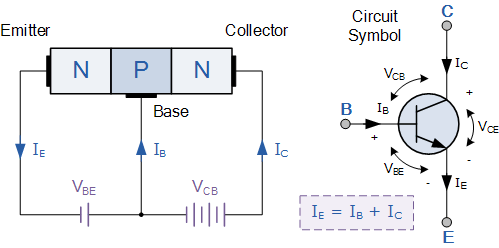
\includegraphics[width=.6\textwidth]{Transistor}
  \caption{Ströme im Transistor}
\end{figure}

\begin{figure}[H]
  \centering
  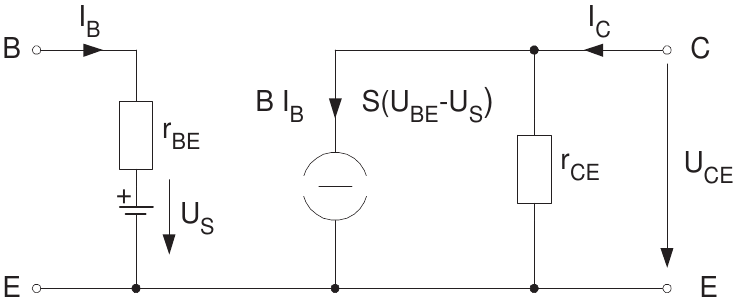
\includegraphics[width=.6\textwidth]{ESBTransistor}
  \caption{Ersatzschaltbild eines Bipolartransistors}
\end{figure}
\mybfcol{Achtung: Beim Zeichnen des Ersatzschaltbildes wird die Spannungsquelle kurzgeschlossen! Das heißt überall wo vorher die Versorgungsspannung war ist nun GND.}

\textbf{Emitterstrom}
\[I_E = I_B + I_C\]

\textbf{Stromverstärkung}
\[I_C = \beta \cdot I_B\]

\textbf{Verlustleistung}
\[P = U_{CE} \cdot I_C\]

\textbf{Steilheit}
\[S = \frac{\Delta I_C}{\Delta U_{BE}} = \frac{I_C}{U_T}\]

\begin{figure}[H]
  \centering
  \includegraphics[width=.6\textwidth]{TransistorVerstärkerschaltung}
\end{figure}

\begin{figure}[H]
  \centering
  \includegraphics[width=\textwidth]{TransistorVerstärkerschaltung_Spannungen}
\end{figure}

\begin{figure}[H]
  \centering
  \includegraphics[width=\textwidth]{TransistorVerstärkerschaltung_OptimalAusgesteuert}
\end{figure}

\textbf{Optimale Spannungsaussteuerbarkeit}

Spannungen sind im Gleichgewicht
\[U_C = U_E = \frac{1}{2} \cdot U_{\text{Bat}}\]
\(U_{\text{Bat}}\) wird immer vollständig auf \(U_C\) und \(U_E\) aufgeteilt.
\[U_{\text{Bat}} = U_C + U_E\]


\end{document}


%%% Local Variables:
%%% mode: latex
%%% TeX-master: t
%%% End:
